\item \points{3b} Implement your approach by completing the
\texttt{initial\_state}, \texttt{predict}, and \texttt{update\_state} methods
of \texttt{src-perceptron/submission.py}.


We provide two kernels, a dot-product kernel and a
radial basis function (RBF) kernel. 

Run \texttt{src-perceptron/submission.py} to train
kernelized perceptrons on \texttt{src-perceptron/train.csv}. The code will then test
the perceptron on \texttt{src-perceptron/test.csv} and save the resulting
predictions in the \texttt{src-perceptron} folder. Plots will also be saved in
\texttt{src-perceptron}.

The output plot should look similar to the following (no plot submission is required):
\begin{figure}[H]
	\centering
	\vspace{2mm}
	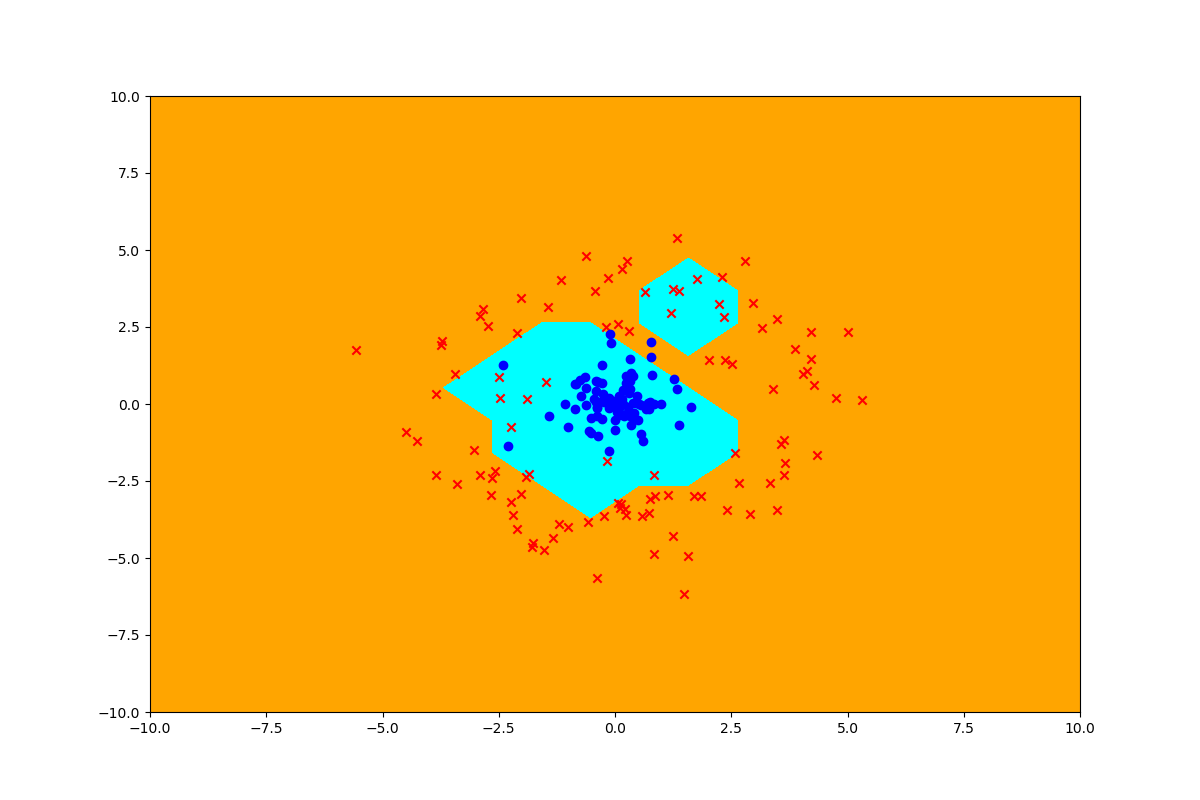
\includegraphics[width=0.65\linewidth]{03-perceptron/perceptron_rbf_output.png}
    \caption{Perceptron classifier plot for radial basis function kernel (Note: This is for reference only. You are not required to submit a plot.)}
\end{figure}

\begin{figure}[H]
	\centering
	\vspace{2mm}
	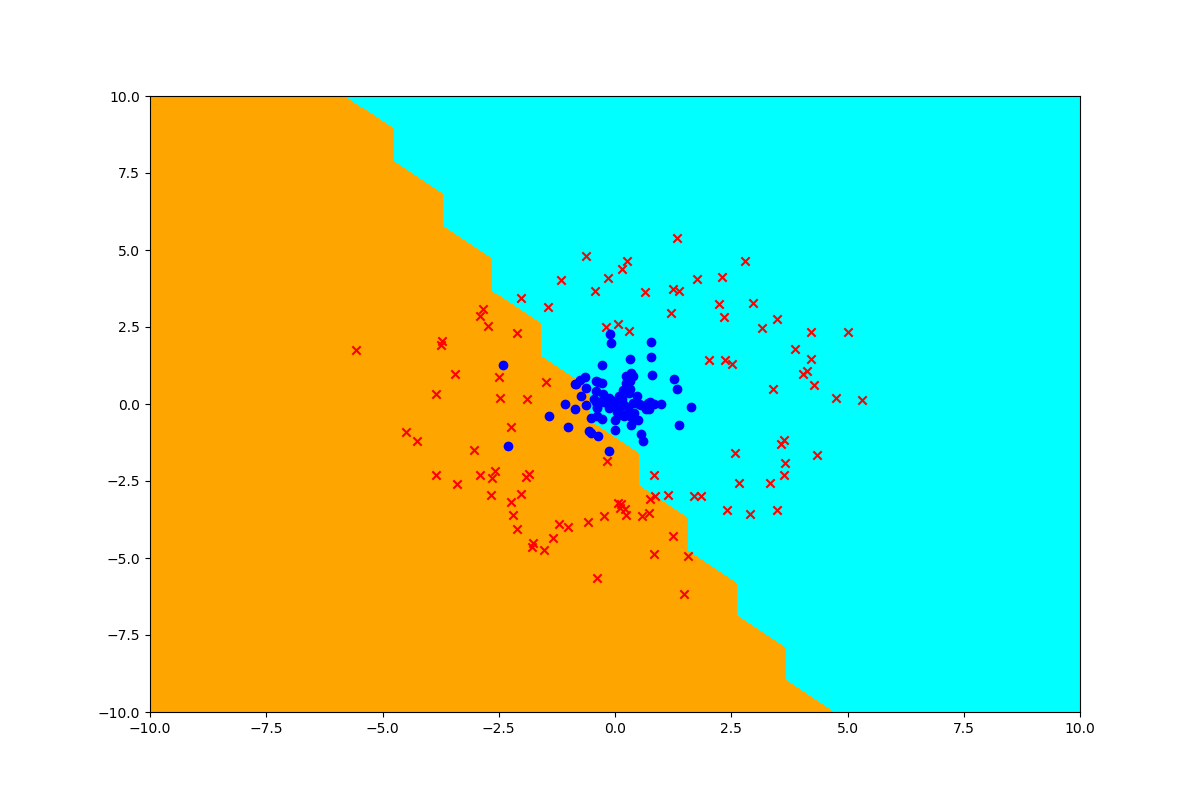
\includegraphics[width=0.65\linewidth]{03-perceptron/perceptron_dot_output.png}
    \caption{Perceptron classifier plot for dot-product kernel (Note: This is for reference only. You are not required to submit a plot.)}
\end{figure}